\documentclass[journal,12pt,twocolumn]{IEEEtran}

\usepackage{setspace}
\usepackage{gensymb}

\singlespacing

\usepackage[cmex10]{amsmath}
\usepackage{amsthm}
\usepackage{mathrsfs}
\usepackage{txfonts}
\usepackage{stfloats}
\usepackage{bm}
\usepackage{cite}
\usepackage{cases}
\usepackage{subfig}
\usepackage{longtable}
\usepackage{multirow}
\usepackage{mathtools}
\usepackage{steinmetz}
\usepackage{tikz}
\usepackage{circuitikz}
\usepackage{verbatim}
\usepackage{tfrupee}
\usepackage[breaklinks=true]{hyperref}
\usepackage{tkz-euclide} % loads  TikZ and tkz-base
%\usetkzobj{all}
\usetikzlibrary{calc,math}
\usepackage{listings}
    \usepackage{color}                                            %%
    \usepackage{array}                                            %%
    \usepackage{longtable}                                        %%
    \usepackage{calc}                                             %%
    \usepackage{multirow}                                         %%
    \usepackage{hhline}                                           %%
    \usepackage{ifthen}                                           %%
  %optionally (for landscape tables embedded in another document): %%
    \usepackage{lscape}     
\usepackage{multicol}
\usepackage{chngcntr}
\DeclareMathOperator*{\Res}{Res}
\renewcommand\thesection{\arabic{section}}
\renewcommand\thesubsection{\thesection.\arabic{subsection}}
\renewcommand\thesubsubsection{\thesubsection.\arabic{subsubsection}}

\renewcommand\thesectiondis{\arabic{section}}
\renewcommand\thesubsectiondis{\thesectiondis.\arabic{subsection}}
\renewcommand\thesubsubsectiondis{\thesubsectiondis.\arabic{subsubsection}}

\newcommand{\bignorm}[1]{\Bigl \| #1 \Bigr \| #1}
\newcommand{\norm}[1]{\| #1 \|}
% correct bad hyphenation here
\hyphenation{op-tical net-works semi-conduc-tor}
\def\inputGnumericTable{}                                 %%

\lstset{
frame=single, 
breaklines=true,
columns=fullflexible
}
\usepackage{graphicx}

\begin{document}
\begin{center}
\huge Challenge 1\\

\large Shaik Zeeshan Ali\\
\large AI20MTECH11001\\
\end{center}
\vspace{0.5cm}
\begin{abstract}
This document explains how to find points on two skew lines where the distance is shortest.
\end{abstract}
\vspace{0.5cm}
Download all python codes from 
\begin{lstlisting}
https://github.com/Zeeshan-IITH/IITH-EE5609/new/master/codes
\end{lstlisting}
%
and latex-tikz codes from 
\begin{lstlisting}
https://github.com/Zeeshan-IITH/IITH-EE5609
\end{lstlisting}
%
\section{problem}
Find the points on two skew lines where the distance between the lines is shortest\\
\begin{align}
    L_1\colon \bm{x}= x_1+\lambda_1\bm{v_1}\\
    L_2\colon \bm{x}= x_2+\lambda_2\bm{v_2}
\end{align}
\section{Construction}
Let $\bm{a}$,$\bm{b}$ be two points on the lines $L_1$,$L_2$ respectively,where the distance $\norm{\bm{a}-\bm{b}}$ is shortest.\\
The vector along the line $(\bm{a}-\bm{b})$ will be parallel to $\bm{v_1}\times\bm{v_2}$\\
\begin{align}
    \bm{a}=x_1+\lambda_1\bm{v_1}\\
    \bm{b}=x_2+\lambda_2\bm{v_2}
\end{align}
The vector along the line $\bm{ab}$ will be \\
\begin{align}
    \bm{ab}=x_1+\lambda_1\bm{v_1}-x_1-\lambda_1\bm{v_1}\notag\\
    \bm{ab}=\begin{pmatrix}x_1 & \bm{v_1}\end{pmatrix}\begin{pmatrix}1 \\ \lambda_1\end{pmatrix}-\begin{pmatrix}x_2 & \bm{v_2}\end{pmatrix}\begin{pmatrix}1 \\ \lambda_2\end{pmatrix}
\end{align}
\section{explanation}
The vectors $\bm{v_1}$,$\bm{v_2}$ are both perpendicular to the line $\bm{ab}$.So the dot product of $\bm{v_1}$,$\bm{v_2}$ with the line $\bm{ab}$ is zero.\\
The dot product of $\bm{v_1}$ with the line $\bm{ab}$ is
\begin{align}
    \bm{v_1^T}\begin{pmatrix}x_1 & \bm{v_1}\end{pmatrix}\begin{pmatrix}1 \\ \lambda_1\end{pmatrix}-\bm{v_1^T}\begin{pmatrix}x_2 & \bm{v_2}\end{pmatrix}\begin{pmatrix}1 \\ \lambda_2\end{pmatrix}=0
\end{align}
The dot product of $\bm{v_2}$ with the line $\bm{ab}$ is\\
\begin{align}
    \bm{v_2^T}\begin{pmatrix}x_1 & \bm{v_1}\end{pmatrix}\begin{pmatrix}1 \\ \lambda_1\end{pmatrix}-\bm{v_2^T}\begin{pmatrix}x_2 & \bm{v_2}\end{pmatrix}\begin{pmatrix}1 \\ \lambda_2\end{pmatrix}=0
\end{align}
Rearranging the equations $(5)$ and $(6)$ in matrix form we get\\
\begin{align}
    \begin{pmatrix}\bm{v_1^T}x_1 & \bm{v_1^T}\bm{v_1} & -\bm{v_1^T}x_2 & -\bm{v_1^T}\bm{v_2}\\\bm{v_2^T}x_1 & \bm{v_2^T}\bm{v_1} & -\bm{v_2^T}x_2 & -\bm{v_2^T}\bm{v_2}\end{pmatrix}\begin{pmatrix}1\\\lambda_1\\1\\\lambda_2\end{pmatrix}=0
\end{align}
simplifying it further\\
\begin{align}
    \begin{pmatrix}\bm{v_1^T}\bm{v_1} & -\bm{v_1^T}\bm{v_2}\\\bm{v_2^T}\bm{v_1} &  -\bm{v_2^T}\bm{v_2}\end{pmatrix}\begin{pmatrix}\lambda_1\\\lambda_2\end{pmatrix}=\begin{pmatrix}\bm{v_1^T}(x_2-x_1)\\\bm{v_2^T}(x_2-x_1)\end{pmatrix}
\end{align}
Solving the equation $(9)$ we get the values of $\lambda_1$ and $\lambda_2$.Substituting the values of $\lambda_1$ and $\lambda_2$ in the equations $(3)$ and $(4)$ we get the values of the point $\bm{a}$ and $\bm{b}$.
\section{example}
Find the points where the distance is shortest between the lines \\
\begin{align}
    L_1\colon \bm{x}= \begin{pmatrix}1\\2\\1\end{pmatrix}+\lambda_1\begin{pmatrix}1\\-1\\1\end{pmatrix}\notag\\
    L_2\colon \bm{x}= \begin{pmatrix}2\\-1\\-1\end{pmatrix}+\lambda_2\begin{pmatrix}2\\1\\2\end{pmatrix}\notag
\end{align}
Using the above equation (9) to solve we get the points as $\frac{1}{12}\begin{pmatrix}27\\-3\\27\end{pmatrix}$ and $\frac{1}{12}\begin{pmatrix}10\\-19\\-26\end{pmatrix}$ as shown in the figure\\
\begin{center}
    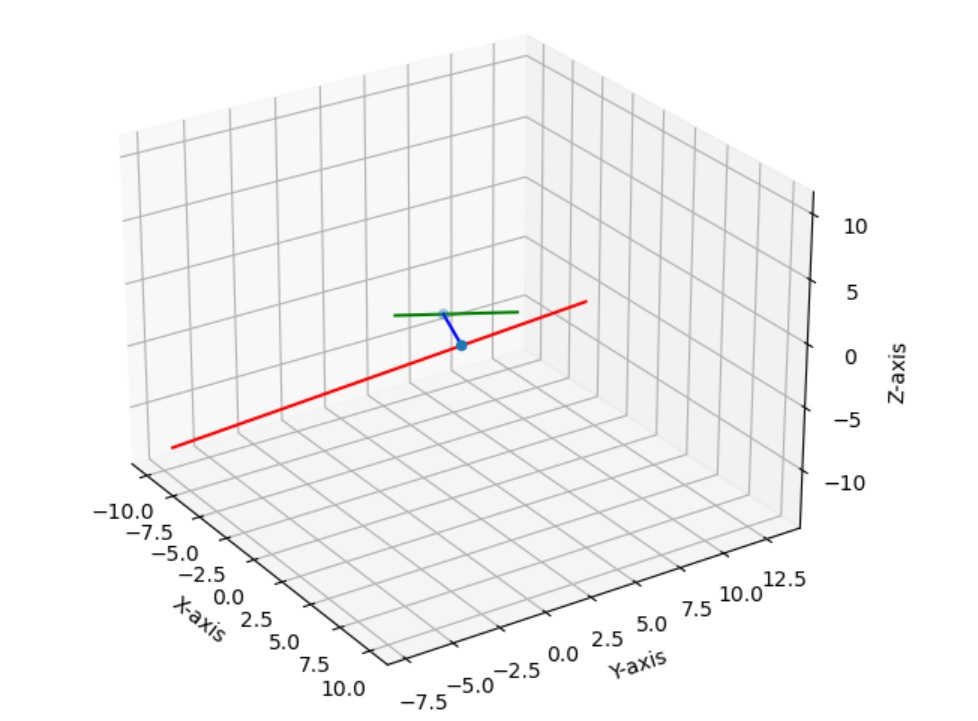
\includegraphics[width=11cm]{assignment2.jpg}
\end{center}

\end{document}
